% !TEX TS-program = xelatex
%
\documentclass[t]{beamer}

\usepackage{lmodern}
\usepackage{textcomp}
\usetheme{metropolis} % https://github.com/matze/mtheme

\usepackage{multirow}

\usepackage[T1]{fontenc}
\usepackage[utf8]{inputenc}

\usepackage[ngerman]{babel}
\usepackage[ngerman]{isodate}

\usepackage{graphicx}
\graphicspath{{assets/}}

\usepackage[export]{adjustbox}

\title{SOCKSv5 (RFC 1928)}
\author{Michael Kaltschmid und Markus Reiter}
\date{\printdate{2017-06-13}}

\usepackage{ragged2e}

\begin{document}
  \RaggedRight

  \maketitle

  \begin{frame}{Problem}
    \begin{itemize}
      \item Es gibt keine Möglichkeit zur transparenten Durchquerung einer Firewall.
      \item Es gibt keine Möglichkeit zur sicheren Authentifikation einer solchen Durchquerung.
    \end{itemize}
  \end{frame}

  \begin{frame}{Was sind Sockets?}
    \begin{itemize}
      \item vom Betriebssystem bereitgestellt
      \item Kommunikationsendpunkt
      \item Austausch von Daten
    \end{itemize}
  \end{frame}

  \begin{frame}{Ansatz - Ablauf TCP}
    \begin{itemize}
      \item
        Client sendet Anfrage mit Versions-Identifikator \\
        und Authentifizierungmethoden:
        \begin{adjustbox}{max width=\textwidth}

          \begin{tabular}{|c|p{4cm}|p{4cm}|}
            \hline
            \texttt{VER} & \texttt{NMETHODS}                      & \texttt{METHODS} \\
            \hline
            \texttt{05}  & Anzahl der Oktetts in \texttt{METHODS} & 1 – 255 Methoden-Oktetts \\
            \hline
          \end{tabular}
        \end{adjustbox}
      \item
        Server wählt eine Methode in \texttt{METHODS} aus, und antwortet:
        \begin{adjustbox}{max width=\textwidth}
          \begin{tabular}{|c|p{8cm}|}
            \hline
            \texttt{VER} & \texttt{METHOD} \\
            \hline
            \texttt{05}  & Ein Oktett aus \texttt{METHODS}, oder \texttt{FF}, falls keine Methode akzeptabel ist. \\
            \hline
          \end{tabular}
        \end{adjustbox}
      \item
        Client schlie{\ss}t die Verbindung, falls er \texttt{FF} als Antwort erhält.
        Sonst wird eine Methoden-spezifische Authentifizierung gestartet.
    \end{itemize}
  \end{frame}

  \begin{frame}{Ansatz - Ablauf TCP}
    \begin{itemize}
      \item
        Client sendet Request-Details:
        \begin{adjustbox}{max width=\textwidth}
          \begin{tabular}{|c|c|c|c|c|c|}
            \hline
            \texttt{VER} & \texttt{CMD}                & \texttt{RSV}         & \texttt{ATYP}            & \texttt{DST.ADDR} & \texttt{DST.PORT} \\
            \hline
            \texttt{05}  & \begin{tabular}{@{}l@{}}
                             \texttt{01} CONNECT \\ 
                             \texttt{02} BIND  \\ 
                             \texttt{03} UDP ASSOCIATE
                           \end{tabular}               & \texttt{00} RESERVED & \begin{tabular}{@{}l@{}}
                                                                                  \texttt{01} IPv4 \\ 
                                                                                  \texttt{03} Domain \\ 
                                                                                  \texttt{04} IPv6
                                                                                \end{tabular}            & Adresse           & Port \\
            \hline
          \end{tabular}
        \end{adjustbox}
      \item
        Server verarbeitet Request und antwortet:
        \begin{adjustbox}{max width=\textwidth}
          \begin{tabular}{|c|c|c|c|c|c|}
            \hline
            \texttt{VER} & \texttt{REP}                & \texttt{RSV}         & \texttt{ATYP}            & \texttt{BND.ADDR} & \texttt{BND.PORT} \\
            \hline
            \texttt{05}  & \begin{tabular}{@{}l@{}}
                             \texttt{00} succeeded \\
                             \texttt{01} general SOCKS server failure \\
                             \texttt{02} connection not allowed by ruleset \\
                             \texttt{03} Network unreachable \\
                             \texttt{04} Host unreachable \\
                             \texttt{05} Connection refused \\
                             \texttt{06} TTL expired \\
                             \texttt{07} Command not supported \\
                             \texttt{08} Address type not supported \\
                             \texttt{09} – \texttt{FF} unassigned \\
                           \end{tabular}               & \texttt{00} RESERVED & \begin{tabular}{@{}l@{}}
                                                                                  \texttt{01} IPv4 \\ 
                                                                                  \texttt{03} Domain \\ 
                                                                                  \texttt{04} IPv6
                                                                                \end{tabular}            & Adresse           & Port \\
            \hline
          \end{tabular}
        \end{adjustbox}
    \end{itemize}
  \end{frame}

	\begin{frame}{Ansatz - Ablauf UDP}
		\begin{itemize}
			\item Client sendet UDP Datagram an spezifierten Port.
			\item Server entweder verwirft Anfrage oder sendet das entsprechendes Datagram zurück. \\
			keine Benachrichtigung in beiden Fällen.
		\end{itemize}
	\end{frame}

  \begin{frame}{Notwendige Details - UDP Header}
    \begin{itemize}
      \item
       UDP Request header: \\
       \begin{adjustbox}{max width=\textwidth}
         \begin{tabular}{|c|c|c|c|c|c|}
          \hline
            \texttt{RSV} & \texttt{FRAG}                & \texttt{ATYP}         & \texttt{DST.ADDR}            & \texttt{DST.PORT} & \texttt{DATA} \\
          \hline
            2 & 1 & 1 & Variable & 2 & Variable \\
          \hline
        \end{tabular}
      \end{adjustbox}
      und Feldern: \\
      \begin{adjustbox}{max width=\textwidth}
        \begin{tabular}{|c|c|c|c|c|c|}
          \hline
            \texttt{RSV}        & \texttt{FRAG}         & \texttt{ATYP}           & \texttt{DST.ADDR}     & \texttt{DST.PORT}     & \texttt{DATA} \\
          \hline
            \texttt{Reserved X'0000'} & \texttt{fragment number} & \begin{tabular}{@{}l@{}}
                                                                  	\texttt{01} IPv4 \\ 
                                                                  	\texttt{03} Domain \\ 
                                                                  	\texttt{04} IPv6
                                                                   \end{tabular} & \texttt{destination address} & \texttt{destination port} & \texttt{data} \\
          \hline
        \end{tabular}
      \end{adjustbox}
    \end{itemize}
  \end{frame}

  \begin{frame}{Notwendige Details - Schichtenmodell}
		\begin{align*}
			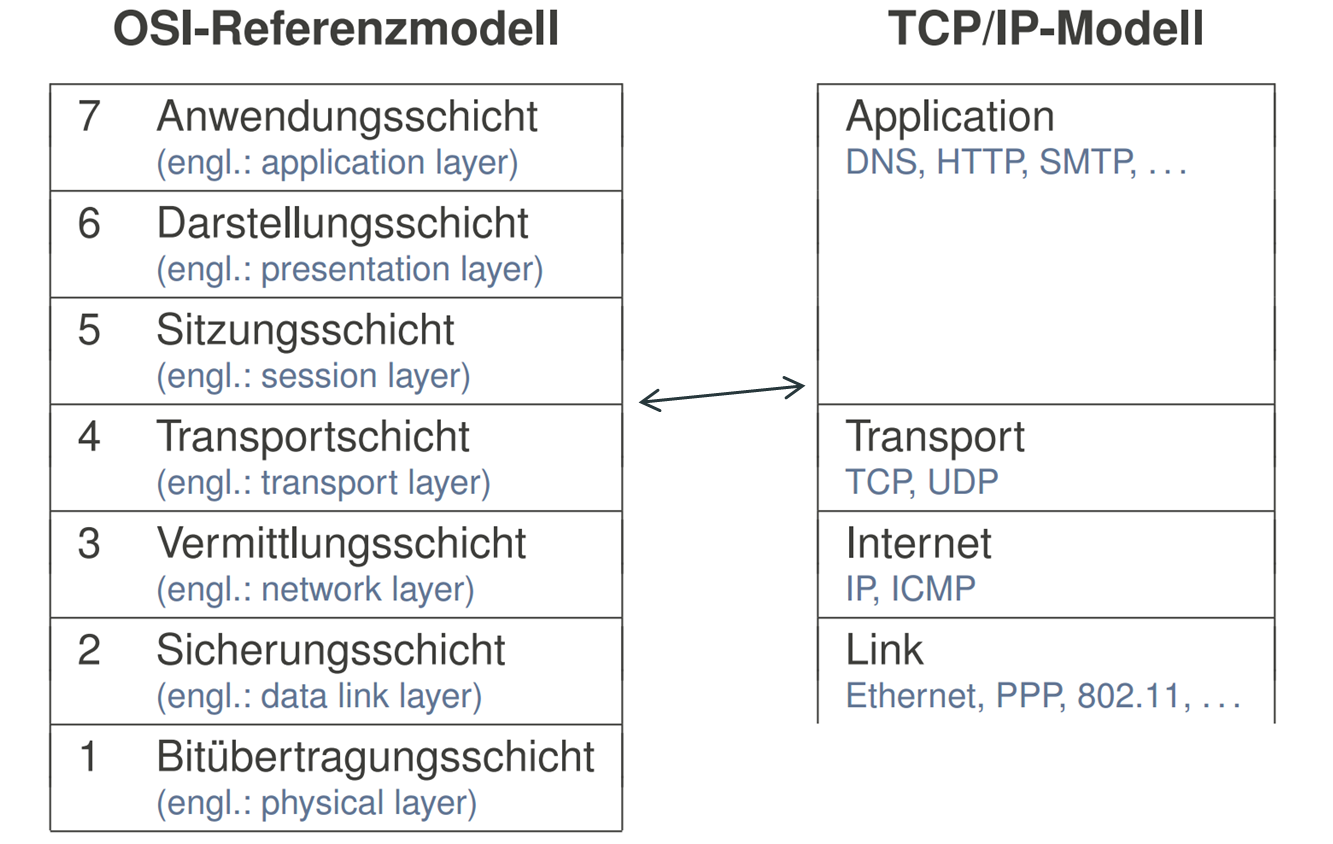
\includegraphics[height=6cm]{schichtenmodell-v2.png}
		\end{align*}
	\end{frame}

  \begin{frame}{Änderungen von SOCKSv4 zu SOCKSv5}
	 \begin{itemize}
		\item
		Auflösung von Domains
		\item
		Kommunikation mittels UDP
		\item
		Unterstützung von IPv6
		\item
		Verwendbar mit sicherer / stärkerer Authentifizierung
  	\end{itemize}
  \end{frame}

  \begin{frame}{Ausblick}
    Verwandte RFCs:

    \begin{itemize}
      \item RFC 3089: SOCKSv5-based IPv6/IPv4 Gateway Mechanism
      \item RFC 1929: Username/Password Authentication for SOCKSv5
      \item RFC 1961: GSS-API Authentication Method for SOCKSv5
    \end{itemize}
  \end{frame}
\end{document}
